\documentclass[runningheads,a4paper]{llncs}

\usepackage[latin1]{inputenc}
\usepackage{amssymb}
\usepackage{amsmath}
\setcounter{tocdepth}{3}
\usepackage{graphicx}
\usepackage{multirow}
\usepackage{rotating}
%\usepackage{subfigure}
%\usepackage{subfig}
\usepackage{url}
\usepackage{caption}
\usepackage{subcaption}
\captionsetup{compatibility=false}

\newcommand{\keywords}[1]{\par\addvspace\baselineskip
\noindent\keywordname\enspace\ignorespaces#1}
\captionsetup[table]{skip=10pt}

\providecommand{\tabularnewline}{\\}

\begin{document}

\mainmatter
\title{Procedural massive monomythic backstories generation using genetic algorithms, autonomous agents and logical reasoning}


\titlerunning{}

%\author{R. H. P. Garc\'ia-Ortega \and P. Garc\'ia-S\'anchez \and J.J. Merelo}
\author{Mustrum Ridcully\inst{1}}
% �Se puede ayudar aqu�?
%
%\authorrunning{R. H. P. Garc\'ia-Ortega et al.}
\authorrunning{}
% (feature abused for this document to repeat the title also on left hand pages)

% the affiliations are given next; don't give your e-mail address
% unless you accept that it will be published
%\institute{Dept. of Computer Architecture and Technology, University
%of Granada, Spain}
\institute{Unseen University of Ankh-Morpork}

%
% NB: a more complex sample for affiliations and the mapping to the
% corresponding authors can be found in the file "llncs.dem"
% (search for the string "\mainmatter" where a contribution starts).
% "llncs.dem" accompanies the document class "llncs.cls".
%




\maketitle

%
%%%%%%%%%%%%%%%%%%%%%%%%%%%%%%%   ABSTRACT   %%%%%%%%%%%%%%%%%%%%%%%%%%%%%%%
%
\begin{abstract}
The procedural generation of massive subplots and backstories in secondary characters that inhabit Open World videogames usually lead to stereotyped characters that act as mere decoration of the virtual world; however, many game designers claim that the stories can be very relevant for the player's experience. For this reason we are looking for a methodology that improves the variability of the characters' personality while enhancing the quality of their backstories following artistic or literary guidelines.
In previous works, we used multi agent systems in order to have stochastic but regulated inter-relations that became backstories; later, we have used genetic algorithms to promote the appearance of high level behaviors inside them.
Our current work follows the previous research line and propose a three layered system (Evolutionary computation - Agent-Based Model - Logical Reasoner) that is applied to the promotion of the monomyth, commonly known as the hero's journey, a social pattern that constantly appears in literature, films, and videogames. 
As far as we know, there is no previous attempt to model the monomyth as a logical theory, and no attempt to use the sub-solutions for narrating purposes. Moreover, this paper shows for the first time this multi-paradigm three-layered methodology to generate massive backstories. 
Different metrics have been tested in the experimental phase, from those that sum all the monomyth-related tropes to those that promote distribution of archetypes in the characters.

% Results are coming...

\keywords{Procedural generation, monomyth, agent-based model, emergent behavior}
\end{abstract}

%
%%%%%%%%%%%%%%%%%%%%%%%%%%%%%%%   INTRODUCTION   %%%%%%%%%%%%%%%%%%%%%%%%%%%%%%%
%
\section{Introduction}
\label{sec:intro}

Non-player characters (NPC for further references) usually interact with the main player in order to challenge them, offer information to complete their goals or provide life-likeness to a virtual world. Following Szymanezyk et al. in \cite{szymanezyk2011individual}, crowds of NPCs enhance the game-play experience of open-world videogames. that are objective-oriented and open-landscaped videogames, following the classification by \cite{aarseth2005hunt}, where a player can roam freely through a virtual world. 

Open worlds are usually created using Procedural Content Generation (PGC) techniques. Recently, PCG is boosting its popularity, mainly due to two reasons: the cost reduction that the automatic generation implies to the developers, and the re-playability that it offers to the players. As a recent example, \textit{No man's sky}, an indie adventure videogame where planets, fauna and flora are created procedurally, won three Game Critics Awards, including Best Original Game and the Special Commendation for Innovation, in the past Electronic Entertainment Expo 2014, a reference annual trade show for the video game industry\footnote{\url{http://www.gamecriticsawards.com/winners.html}}.

Szymanezyk et al. in \cite{szymanezyk2011individual} remark that virtual humans composing a crowd are often modeled only in terms of individuals and that research in crowd behavior identifies that a large majority of persons in real crowds do not act in individualistic terms. Characters need to explore a social network in order to augment their believability and, as simulated crowds, need to consider group aspects, hence they propose to create a network-type data structure with the help of on-going sociology work.
The different inter-relations between the NPCs generate events and the goal of our research is to use those events to generate quality backstories for the NPCs, that are an important part of the game narrative, as defined by Bateman et al. in \cite{bateman2007game}:

Backstories are the histories leading up to the events of the game, and they give the player the information they need to immerse themselves in the fiction. Since backstories are relevant for the immersion of the game, in this research we create them massively using social interactions between the NPCs.

Archetypes are recurring thematic and linguistic patterns in folklore and literature \cite{garry2005archetypes}. In videogames, archetypes are classically related to the nature of the characters (for example, thief, warrior or wizard), which reminds of the concept of stereotype, the unfair belief that all people or things with a particular characteristic are the same. From our point of view, an archetype is a role that a character plays on a given moment or period, regardless of the nature of characteristics of them. Following this reasoning, a character could play many different archetypes in their life, even at the same time. But, what could be the minimum set of archetypes to design if we want to create interesting backstories? We found a good answer in the monomyth.

The monomyth, commonly known as the hero's journey, is a pattern where different archetypes behave in a specific way and conform to ancient and modern myths from cultures all over the world: It is the story of someone who is considered a hero, that has to deal with his/her shadow, who is waiting at the end of a journey, where different characters appear like mentors, allies or obstacles. The monomyth was studied by Joseph Campbell in The Hero with a Thousand Faces~\cite{campbell2008hero}, and later by Vogler in The writer's journey~\cite{vogler2007writer}. The monomyth has been typically applied to literature and traditional media, but it actually manifests also in modern videogames like Mass Effect or Skyrim \cite{knopf2013rationalist} among others. In videogames, the \textit{monomyth} is used to design the main plots that the player can empathize with: In his work \cite{bartle2004massively}, Bartle identifies and examines the application of key elements of the monomyth to videogames, and discovers that players play virtual worlds as a mean for self-discovery, by subconsciously, following a predetermined path: the monomyth. Our work uses the monomyth as a frame for backstories in videogames, since it provides a basic but omnipresent set of high level behaviors that can be found in the daily life but also in the biggest adventures. We use the monomyth as metric of interest in order to promote the archetypes present in it.

Our research uses a virtual world inhabited by autonomous agents, but the idea of using Agent-Based Models (ABM) of the world to generate stories is not new, as remarked in previous works \cite{garcia2014my} \cite{garciaortega2015how}, especially in the area of the interactive drama.
In 2002, Virtual storyteller \cite{theune2002virtual} used agents that improvised using techniques from improvisational theater, a plot guide and a narrator. Our technique uses the same approach but there is no plot guide agent. Instead, a Genetic Algorithm (GA) guides the mood of the backstories created by finding 'archetypes'.
Mei et al. created in 2005 a system called Thespian \cite{si2005thespian}, where the agents' personalities, their goals, are fitted so that they are motivated to perform according to the scripts. They use lookahead search in a decision-theoretic framework to determine the best way to achieve their goals and they are prepared to respond to the user interaction in a consistent way. Like Thespian, our work is also focused in the final script, not in modeling the agent's personality, but in our target application, open-world videogames, scripts are auto-generated in order to be re-playable.
In 2008, Peinado et al. studied in \cite{peinado2008revisiting} the Belief-Desire-Intention (BDI), a cognitive model that reinforces narrative causality insofar as motivations and where beliefs are causal links that enrich characters. DBI is a theory that is starting to be considered a promising tool for modeling sophisticated characters, but it is not suitable for our research since we need to use more basic agents, easy to model and parametrize: As discussed by Sanchez and Lucas in \cite{sanchez2002exploring}, the analysis of relatively simple simulations using ABMs can, nonetheless, be quite complex, and in our case we use them in massively inhabited virtual worlds hard to analyze and evolve.

In previous works we used Finite State Machines (FSMs) to model the agent behavior, but FSMs and its variants have limitations in developing game Artificial Intelligence (AI), for this reason in our present research we have used Behavior Trees (BT) instead, following Lim's arguments in \cite{lim2009ai}: BTs simplify the design of behavior by allowing the re-usability of tasks without increasing the complexity of the nodes and transitions. Moreover, BTs are the most successful method to model AIs in videogames, and many game engines allow the possibility to create them, like Unity3D or Unreal Engine. A behavior tree consist of different kinds of tasks that are the nodes in a hierarchical structure, following the description by Trembley \cite{tremblay2012understanding}: conditions, that check properties of the environment, actions, that alter the state of the environment,  and compositions, whose result is calculated from the children tasks.

Our previous work has reinforced the idea that a hybrid \textit{Evolutionary Computation - Agent Based Model} (EC-ABM) methodology can be used to achieve the emergence of archetypes, according to the structure studied by Cioffi et al. in \cite{cioffi2012evolutionary}. In our current research, we add a new layer, that is in charge of evaluating the backstories: The Logical Reasoning (LR). We use an ABM for the execution of the virtual world, whose execution is parameterized by a set of integer and float values, a Logical Reasoner that evaluates the events generated by each simulation and a Genetic Algorithm (GA) to find the set of parameters with highest fitness. The LR uses a mixed imperative-declarative paradigm, following Denti's approach in \cite{denti2001tuprolog},  to make high level deductions from the simulation's events, that are also expressed as logical predicates, using a logical theory that is modeled from the monomyth. The three layered architecture proposed can be observed in figure~\ref{fig:3_layered}.

% Pending some review comments from the original document in drive

%
%%%%%%%%%%%%%%%%%%%%%%%%%%%%%%  METHODOLOGY  %%%%%%%%%%%%%%%%%%%%%%%%%%%%%
%
\section{A backstory generator that promotes the monomyth}

In this section we will present a system that uses the three-layered system EC-ABM-LR to generate and evaluate backstories in the virtual world. Firstly, in section \ref{sec:architecture}, we show the high level architecture of the system and the tasks assigned tof each logical module. Later, in section \ref{sec:abm} we give the details of the ABM layer including the virtual world, the agent's model, the parameterization of the simulation and the output format. Then, in section \ref{sec:lr}, we propose an implementation of the logical model of the monomyth, and a method to evaluate the quality of the backstories using logical reasoning on that model. Finally, in section \ref{sec:ec}, we argue the usage of a GA to promote the emergence of the monomyth.

\subsection{The system architecture}
\label{sec:architecture}

\begin{figure}[t]
	\centering
	\begin{subfigure}[b]{0.33\textwidth}
		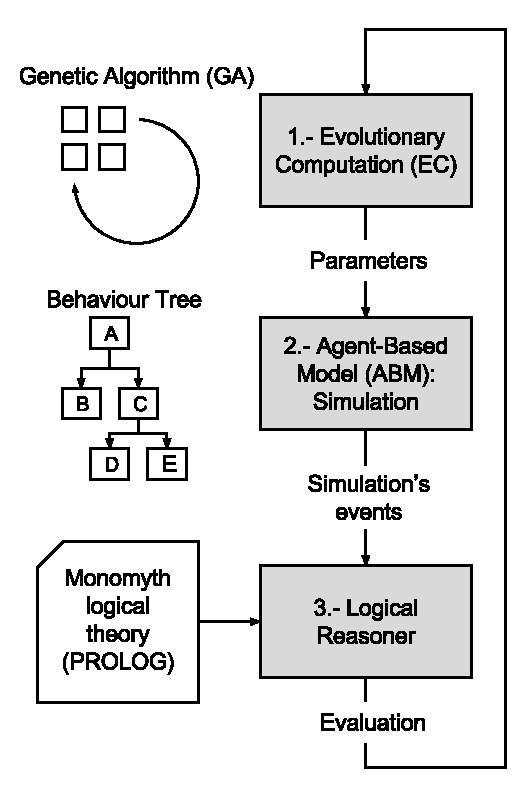
\includegraphics[width=\textwidth]{3_layers.pdf}
		\caption{Proposed three-layered architecture (EC-ABM-LR).}
		\label{fig:3_layered}
	\end{subfigure}
	~
	\begin{subfigure}[b]{0.63\textwidth}
		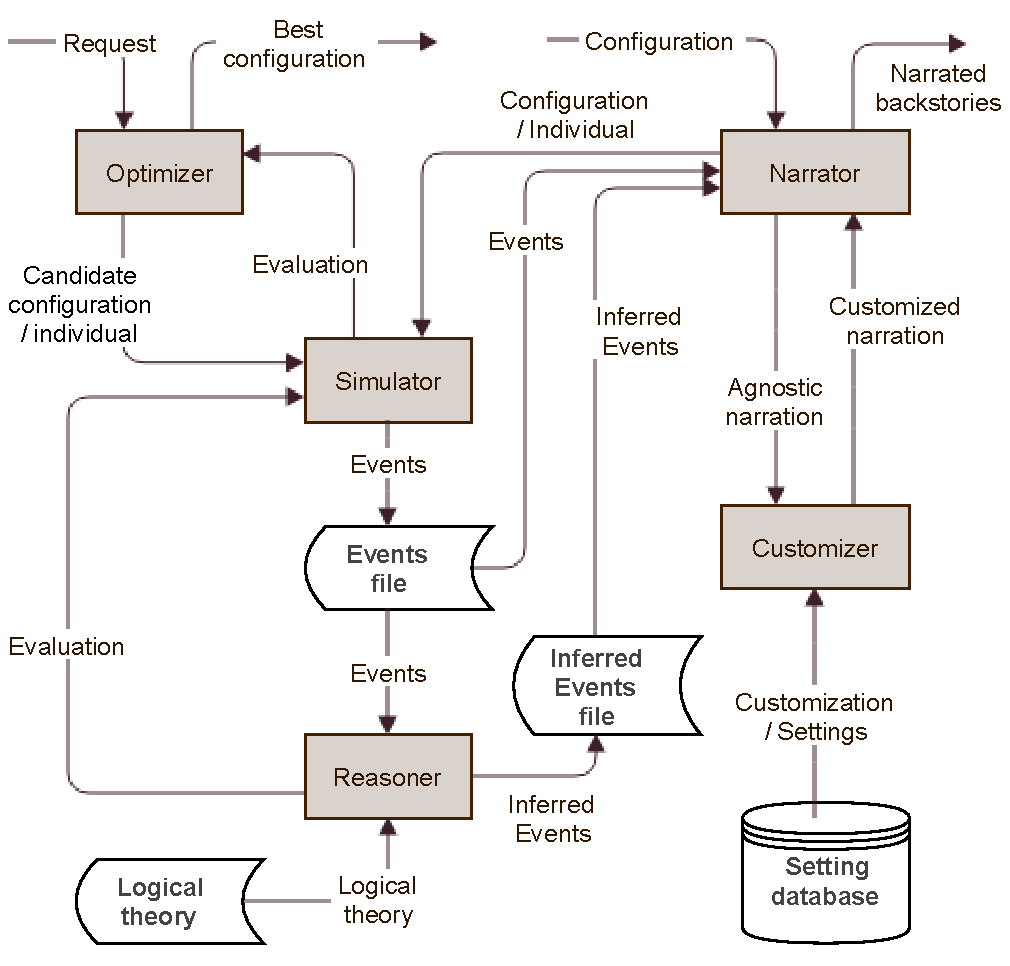
\includegraphics[width=\textwidth]{made_architecture.pdf}
		\caption{Proposed components and data flow diagram of the whole architecture.}
		\label{fig:dataflow}
	\end{subfigure}
	\caption{high-level architecture of the system.}
\end{figure}

The proposed system is described in the Dataflow Diagram of figure \ref{fig:dataflow}. Different modules have been defined: The optimizer, the simulator, the reasoner, the narrator and the customizer. The Optimizer, formerly the EC layer, uses a GA whose individuals are simulation configurations and returns the best individual found. The fitness function of each individual consists in several simulations, performed by the Simulator, i.e. the ABM layer, that uses a multi-agent system in order to generate a sequence of events. These events are evaluated by the LR, the third layer, that uses predicate logic to assign a numerical value to the events following guidelines extracted from the monomyth. The Simulator runs the virtual environment with each configuration in different trials and returns the average (the fitness) to the Optimizer. On the other hand, the Narrator takes a given solution and transforms it to an agnostic narration, that is a selection of relevant predicates without final names for the narration elements. The Customizer is in charge of assigning names and structures to the agnostic narration in order to apply a specific literary setting, for example, middle-age, futuristic, steampunk or Shakespearian.


\subsection{An agent-based model that generates simple events}
\label{sec:abm}

The virtual environment that we propose in this work is called ColourForms, and has been designed as a board-like game that focuses in the four independent, ontic dimensions that conform the ludo-narrative design space described by Aarseth in his work \cite{aarseth2012narrative}: world, objects, agents and events. In our virtual environment, pieces will compete and collaborate in order to reach their desired colour. The narrative, as Aylett studied in \cite{aylett1999narrative}, emerges through small interactions between the characters. The main elements are described as follows: 

\begin{description}
	\item[{\bf World}]: Our backstories need spatio-temporal dimensions, namely, a place where they occur and a time that sequences and orders the events. In Colourforms, we propose to use a very simple map: the checkerboard, that consist of 64 squares (8x8). The time is measured in virtual days.
	\item[{\bf Agents}]: Our agents are pieces that can occupy one cell each. There are three shapes for the pieces (circle, square and triangle) and a zero-sum game relation between them, rock-paper-scissors alike, in order to establish a method to decide the winner and the loser in individual direct conflicts while keeping a global balance. Agents change along the timeline: every piece has a background color and a foreground color that are constantly modified. The background color varies randomly in a slowly way for every piece and represents the continuous internal changes in the character needs. The foreground color can be changed by the piece or by other pieces under certain circumstances and is used to improve the happiness: the piece is happier when the two colours are equal. 
	\item[{\bf Objects}]: We use one type of object, that the characters compete and collaborate for: the color spot. In our environment, the agents can stain with the spot in order to become colored. The color spots can appear or disappear from the world randomly.
	\item[{\bf Events}]: The characters can interact between them and the environment, although the number of actions is very limited: move to a free adjacent cell, push another agent to a  depending on the shape, interchange the background color and stain with a color spot.
\end{description}

As the introduction remarked, following Szymanezyk et al. in \cite{szymanezyk2011individual}, characters need to explore a social network in order to augment their believability. The social component is defined in ColorForms by an affinity matrix: Each piece has an affinity with every other piece in the board, that will depend on their shape, background and foreground colors. This affinity is dynamic and will take part in the decisions that the piece makes, for instance, the joy of the piece will be influenced by the ones with high affinity with it.

In our proposal, events are represented as logical predicates. Kim \cite{kim1976events} theorized that the term 'event' usually implies a change, and most changes are changes in a substance (an individual, an object, a living thing or a system), that occur when 'it acquires a property it did not previously have, or loses a property it previously had'. Formerly, Kim defined the events in his theory of the structured complexes using the canonical notation [x, P, t], where x is the substance, P is the property it exemplifies and t is the time. The existence condition implies that Event [x, P, t] exists just in case that substance x has the property P at the time t. In our work, the events that compound the backstories are defined as meaningful logical predicates with notation Predicate (t, x\_0, /dots , x\_n) where t is the time, and each x is an element of the world (a character, a cell, a moment, the property of an element or a value). Each predicate has a name, a signature (or arguments) and an interpretation, that is a description of the event in natural language.
Our current research contemplates two types of predicates: Those that have been generated by the agents in the virtual environment (world's facts, present in tables \ref{tab:board_events}, \ref{tab:standard_events}, \ref{tab:conditions} and \ref{tab:strategies})  and those that are inferred using the Reasoner module, related to the monomyth (world's deductions, present in figure \ref{fig:theory}).

The virtual environment created for this work, the pieces (characters) are emotion-driven and can perform different strategies to interact with each other in order to generate events that will conform later backstories. The behavior tree used, described in figure~\ref{fig:bt_autogen}, has condition nodes and action nodes; when a condition is fulfilled it generates an event from the table table~\ref{tab:conditions} and when an action is executed correctly it generates an event from table~\ref{tab:strategies}. Our implementation of behavior tree executes the tree in pre-order until a leaf node is evaluated as 'success'.

\begin{figure}[ht]
	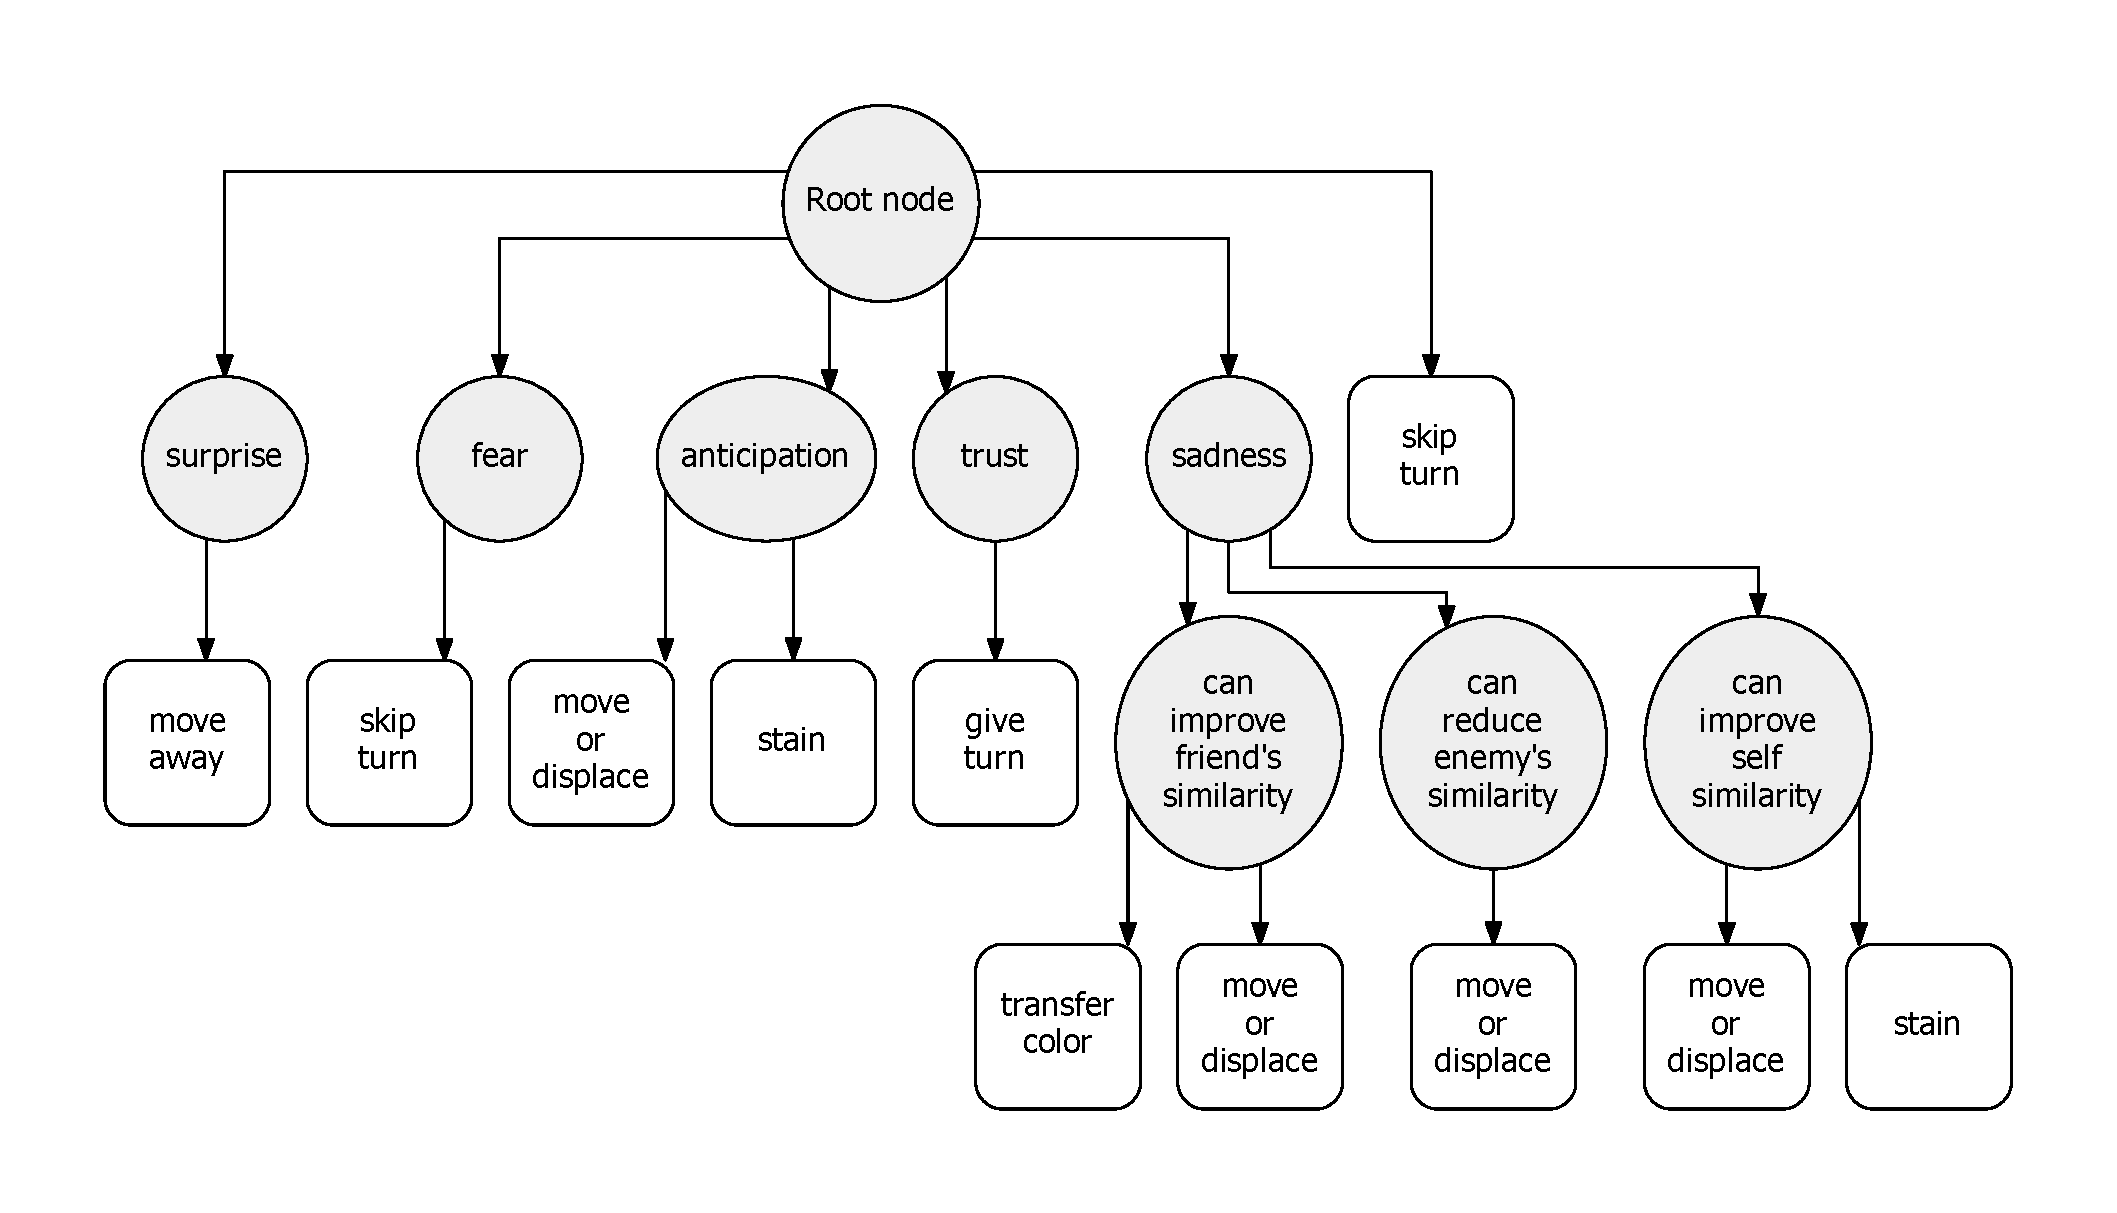
\includegraphics[width=\textwidth]{bt_autogen.pdf}
	\caption{Proposed agents' behavior tree: Circular nodes represent conditions and rectangular nodes represent actions.)}
	\label{fig:bt_autogen}
\end{figure}

\begin{table}[ht]
	\scriptsize
	\begin{center}
		\def\arraystretch{1.5}
		\setlength\tabcolsep{0.1cm}
		\begin{tabular}{| p{4cm} | p{8cm} |}
			\hline
			\textbf{Event signature} & \textbf{Interpretation} \\ \hline
			newDay (Day) & The day \textit{Day} begins \\ 
			\hline
			characterAppears (Day, Subject, Foreground, Background, Shape, Cell) &
			The character \textit{Subject} with shape \textit{Shape}, background color \textit{Background} and foreground color \textit{Foreground} is placed in the cell \textit{Cell} the day \textit{Day} \\
			\hline
			colorSpotAppears (Day, Spot, Color, Cell) &
			The color spot \textit{Spot} with color \textit{Color} is placed in the cell \textit{Cell} the day \textit{Day} \\ 
			\hline
			colorSpotDisappears (Day, Spot) &
			The color spot \textit{Spot} is removed from the board the day \textit{Day}\\ 
			\hline
			areNear (Day, Subject, [CharacterThatIsNear]) &
			The character \textit{subect} is near the characters \textit{CharacterThatIsNear} the day \textit{Day}\\ 
			\hline
		\end{tabular}
		\caption{Events related to the board configuration.}
		\label{tab:board_events}
	\end{center}
	\vspace{-2em}
	\scriptsize
	\begin{center}
		\def\arraystretch{1.5}
		\setlength\tabcolsep{0.1cm}
		\begin{tabular}{| p{4cm} | p{8cm} |}
			\hline
			\textbf{Event signature} & \textbf{Interpretation} \\ \hline
			naturalChange (Day, Subject, OldColor, NewColor)
			& \\ 
			\hline
			isEnemyOf (Day, Subject, [Enemy]) 
			& \\ 
			\hline
			isFriendOf (Day, Subject, [Friend]) 
			& \\ 
			\hline
			joy (Day, Subject, JoyLevel) 
			& \\ 
			\hline
		\end{tabular}
		\caption{Common events for each character's virtual day.}
		\label{tab:standard_events}
	\end{center}
	\vspace{-2em}
	\scriptsize
	\begin{center}
		\def\arraystretch{1.5}
		\setlength\tabcolsep{0.1cm}
		\begin{tabular}{| p{4cm} | p{8cm} |}
			\hline
			\textbf{Event signature} & \textbf{Interpretation} \\ \hline
			canImproveFriendSimilarity (Day, Subject, Friend)
			& \\ 
			\hline
			canImproveSelfSimilarity (Day, Subject, Spot) 
			& \\ 
			\hline
			canReduceEnemySimilarity (Day, Subject, Enemy) 
			& \\ 
			\hline
			hasAnticipation (Day, Subject, Spot)
			& \\ 
			\hline
			hasFear (Day, Subject, Enemy)
			& \\ 
			\hline
			isSad (Day, Subject)
			& \\ 
			\hline
			isSurprised (Day, Subject)
			& \\ 
			\hline
			trusts (Day, Subject, Friend)
			& \\ 
			\hline
		\end{tabular}
		\caption{Events generated by conditions of the Behaviour tree: Character's states.}
		\label{tab:conditions}
	\end{center}
	\vspace{-2em}
	\scriptsize
	\begin{center}
		\def\arraystretch{1.5}
		\setlength\tabcolsep{0.1cm}
		\begin{tabular}{| p{4cm} | p{8cm} |}
			\hline
			\textbf{Event signature} & \textbf{Interpretation} \\ \hline
			displaces (Day,Subject,Enemy,Cell)
			& \\ 
			\hline
			givesTurn (Day, Subject, Friend)
			& \\ 
			\hline
			moves (Day, Subject, Cell)
			& \\ 
			\hline
			movesAway (Day, Subject, Cell)
			& \\ 
			\hline
			skipsTurn (Day, Subject)
			& \\ 
			\hline
			stains (Day, Subject, Spot)
			& \\ 
			\hline
			transfersColor (Day, Subject, Friend)
			& \\
			\hline
		\end{tabular}
		\caption{Events generated by actions of the Behaviour tree: Character's strategies.}
		\label{tab:strategies}
	\end{center}
\end{table}

The Simulator takes an array of 52 values as input, maps them to the environment internal variables and performs the execution of the virtual world by running sequentially the parametrized agents' behavior tree. Finally, when a specific number of virtual days is reached, the simulation finishes and the generated events are sent to the Reasoner for further analysis. The structure of the configuration array and the meaning of each element are described in figure~\ref{fig:abm_parameters}. As we will se in further sections, the configuration array of the Reasoner will be the chromosome in the Optimizer, in other words, the individual of the GA.

\begin{figure}[ht]
	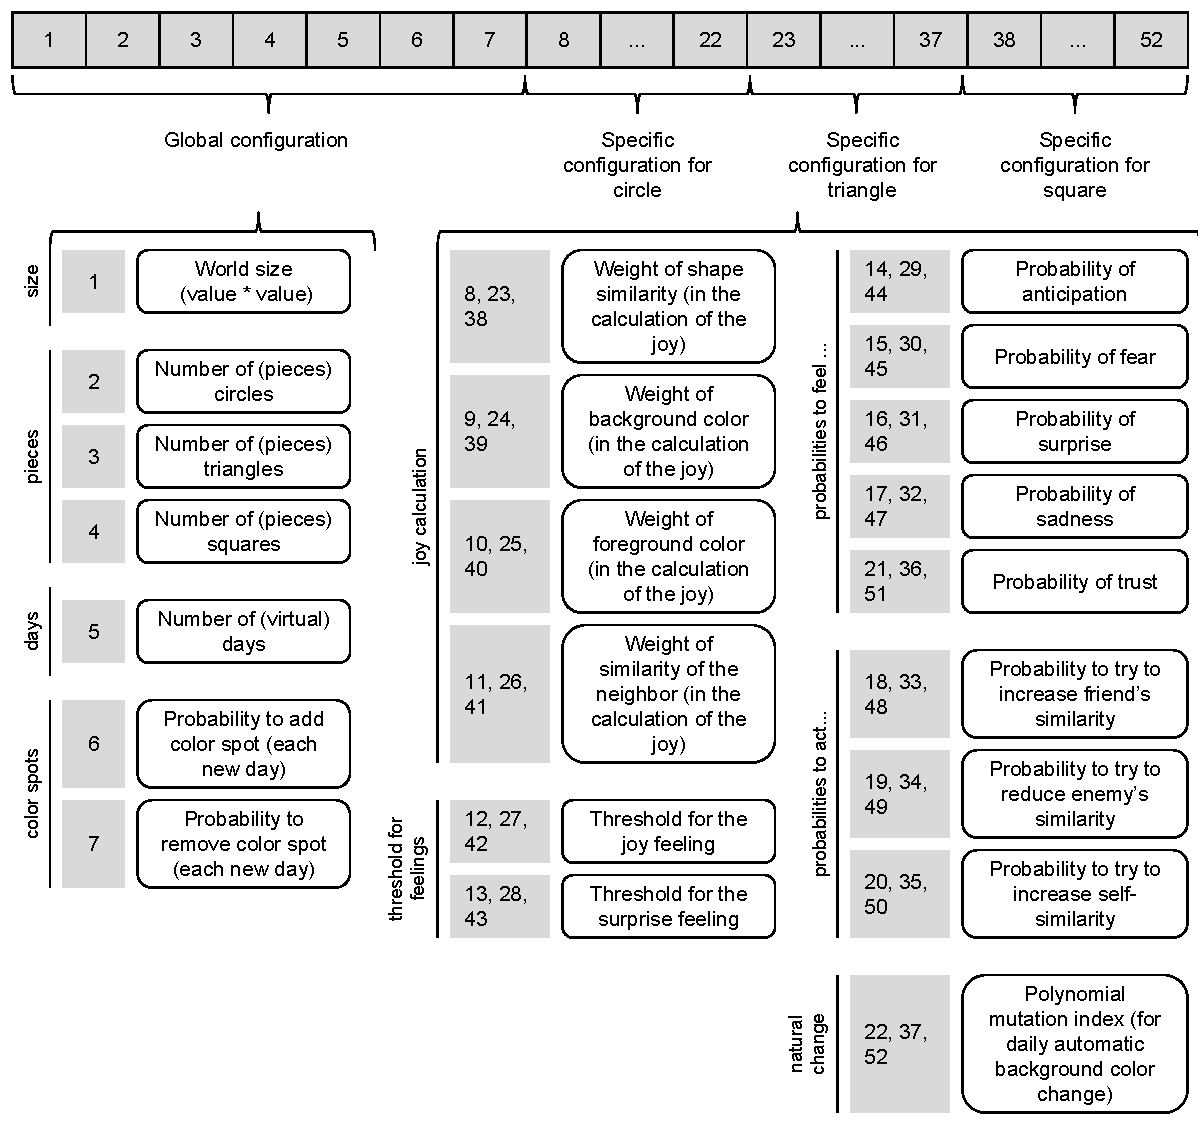
\includegraphics[width=\textwidth]{abm_parameters.pdf}
	\caption{Configuration array of the reasoner (ABM layer) and structure of the individual of the Optimizer (EC layer). Gray rectangles stand for the index of the parameters.}
	\label{fig:abm_parameters}
\end{figure}

\subsection{Construction of the monomyth}
\label{sec:lr}

As remarked in section~\ref{sec:intro}, the monomyth is a pattern that conforms the quintessence of heroism in literature and is composed of different archetypes. Vogler in \cite{vogler2007writer} encountered that archetypes are not 'rigid character roles' but 'flexible character functions' performed to achieve certain effects in the story, hence the same character can play different archetypes along a story.
'There are, of course, many more archetypes; as many as there are human qualities to dramatize in stories', but we will focus in the eight archetypes that conform the monomyth:


\begin{enumerate}
	\item The \textbf{Hero} is willing to sacrifice his own needs on behalf of others.
	\item The \textbf{Mentor} teaches and protects heroes and gives them gifts.
	\item The \textbf{Threshold} Guardians are the the forces that the hero must overcome.
	\item The \textbf{Herald} is the caller to the adventure for the hero.
	\item The \textbf{Shapeshifter} changes (of archetype) along the journey.
	\item The \textbf{Shadow} is the villain or antagonist; the dark side.
	\item The \textbf{Ally} accompanies or helps the hero through the journey.
	\item The \textbf{Trickster} is a mischief-makers.
\end{enumerate}

In our approach, we have taken the archetypes that conform the monomyth and tried to define them in terms of the world's events described in section~\ref{sec:abm}. The Reasoner uses a logical theory in PROLOG, that is a powerful approach since it gives us the possibility to compound predicates and use time-frameworks. The terms in our theory are shown in figure~\ref{fig:theory} in an ordered way following a dependency graph. Coming up next we describe our implementation of the archetypes and other needed concepts.

\begin{enumerate}
	\item We define \textbf{Conflict} as a sequence of events that succeed in a certain moment where two characters take part (the winner and the loser). In the ColorForms game, a conflict might appear when a piece scares or displaces other, or when they takes a color spot that the other desires. If a two pieces are friends and one of them is displaced by a third piece, the two friends have both a conflict with them.
	\item We define \textbf{Journey} as time interval between two conflict between two characters. The first conflict has to be lost by one of them (the \textbf{Hero}) and the second one has to be lost by the other (the \textbf{Shadow}). Moreover, the Shadow must be 'more evil' than the Hero, that is to say that must have helped less friends until this moment.
	\item We define \textbf{Mentor} as a character that is a friend of the Hero during the Journey and helps them at least once. 
	\item We define \textbf{Threshold Guardian} as a character that loses a conflict with the hero along the journey. 
	\item We define \textbf{Herald} as a friend of the hero in a Journey that has the initiator conflict.
	\item We define \textbf{Shapeshifter} as a character that has played the Ally and the Threshold Guardian archetypes in the same Journey.
	\item We define \textbf{Ally} as a character that helps the Hero in a Journey. It can give the Hero an extra turn to accomplish them goals or they can accompany the Hero physically in the map along the journey.
	\item  We define \textbf{Trickster} as a character that accompanies the Hero along the Journey and is trickier. In our implementation, to be trickier tan other can imply to have more joy than them.  
\end{enumerate}


\begin{figure}
	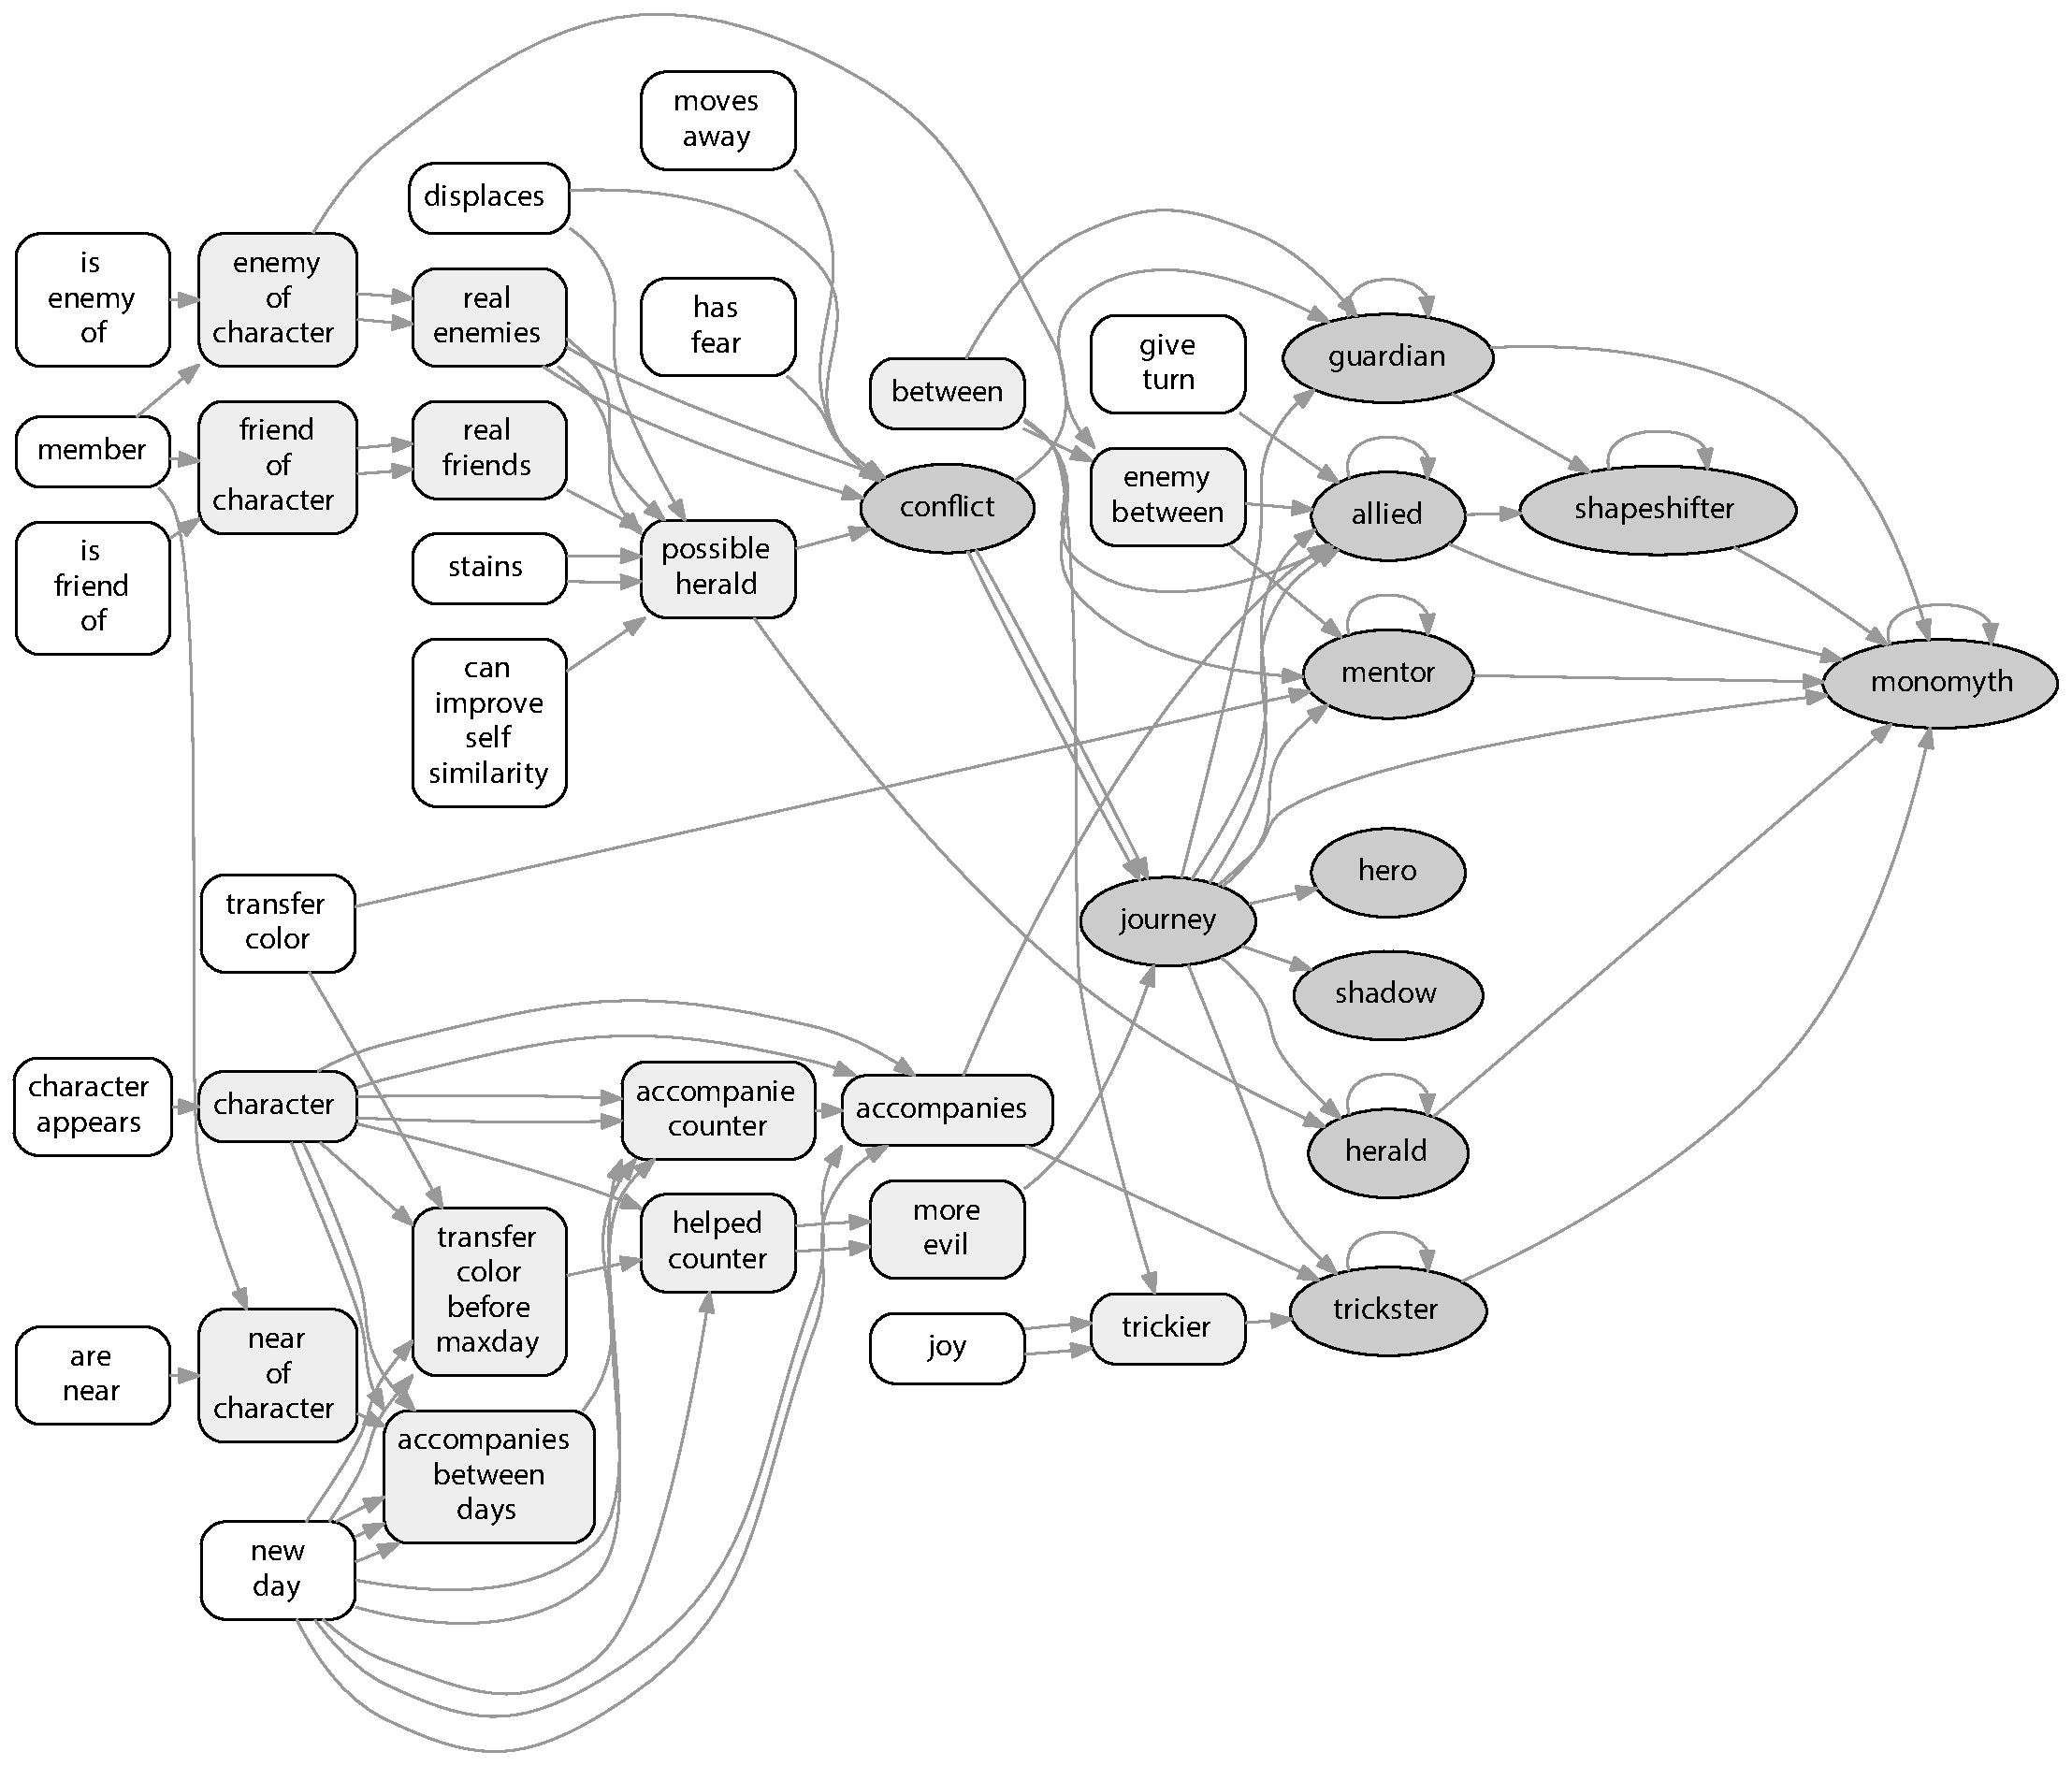
\includegraphics[width=\textwidth]{theory.pdf}
	\caption{Predicate dependencies in the proposed logical theory of the monomyth: White nodes represent predicates generable by the ABM layer and gray predicates are inferred by the Reasoner. Dark-gray predicates conform the monomyth.}
	\label{fig:theory}
\end{figure}

\subsection{Emergence of archetypes}
\label{sec:ec}

% --------------------------------------------------------------


%%%%%%%%%%%%%%%%%%%%%%%%%%  EXPERIMENTS AND RESULTS  %%%%%%%%%%%%%%%%%%%%%%%%%%
%
\section{Experiments and Results}

\section{Conclusions}


\section*{Acknowledgments}
Hidden for double blind review 
%\scriptsize{This work has been supported in part by SIPESCA (Programa Operativo FEDER de Andaluc\'ia 2007-2013), TIN2011-28627-C04-02 (Spanish Ministry of Economy and Competitivity), SPIP2014-01437 (Direcci\'on General de Tr\'afico), PRY142/14 (Fundaci\'on P\'ublica Andaluza Centro de Estudios Andaluces en la IX Convocatoria de Proyectos de Investigaci\'on) and PYR-2014-17 GENIL project (CEI-BIOTIC Granada).}


%
%Hidden for double-blind review


\bibliographystyle{splncs}
\bibliography{made-evostar}


\end{document}
